\chapter{激光致自由域内同相线性三空泡的动力学}

\section{单帧瞬态曝光照相系统和多激光空泡的实现}
\begin{figure}[H]
    \centering
    \includegraphics[width=\linewidth]{img/fig4.1.png}
    \caption{多空泡单帧瞬态曝光阴影法照相的实验设置。}
    \label{fig4.1}
\end{figure}




本作中用于研究激光致对称线性排布的三个同相空泡的实验装置如图 \ref{fig4.1}所示。
为了产生空泡,采用了 1064 脉冲激光波长: 1064nm; 最大单脉冲能量: 1J;
脉宽:10ns)。单脉冲能量从 100mJ 到
1J,激光器能量浮动±5\%。分波片把激光分成两部分。一部分用于监测能量,一部分被三点分波片
(DOE,Diffractive Optical Element; Holo/Or TS-245-I-Y-A)
分成同一平面内等角的三束光束。三个反射镜将三束光反射到一个用于聚焦并获得规则空泡的消球差透镜
($f=30\mathrm {mm}$)
中心。如此,可以在焦平面处获得与反射镜、透镜中心同平面的竖直排列的焦点。在焦点处,水箱
(熔融石英, $50\times 50 \times 50 \mathrm{mm^3}$)
中的去离子水被击穿,并产生等离子体,其后演化成空泡。可以通过遮掩特定的光束来获得单个或者两个空泡。实验中,可以通过改变反射后的激光的入射角度和镜片间的距离来获得不同的焦点距离。

为了对空泡脉动的快速过程进行成像,使用了单帧工业相机 (Imi, imc7017g)
和短脉宽 (Nd: YAG,波长: 1064nm; 脉宽: 2.5 ns) 照明激光。照明激光经过
KTP 晶体倍频获得 532nm
的照明脉冲。照明脉冲经过衰减并扩束。然后,此照明光携带空泡信息照在 CCD
上。探测光与激发光和空泡排列垂直。延迟信号发生器 (Stanford Research
Systems Inc., DG535) 用来触发 CCD
和相机。通过光电二极管能够获得击穿闪光和照明光的时间延迟,以此来获得 CCD
收集到的空泡信息的具体时间。

在实验中,最大空泡的半径通过在空泡阵列实验前的用相同激光能量的孤立球形单空泡实验获得\cite{han_dynamics_2015,fong_interactions_2009}。记录了单空泡的脉动和溃灭时间。实验结果符合 Keller-Miksis
模型。溃灭时间波动±5\%。如此,理想的最大空泡半径 $R_0$
通过溃灭时间的中值而获得 \cite{Kroninger2010}。与通过阴影面积获得的结果
\[R_{\text{0}}=\frac{\sqrt{\text{max(Area)}}}{\pi}\,,\]
比较,差别十分微小,此处忽略之。空泡的初始距离 $D_0$ 通过低于 100ns
的早期帧获得,此时等离子体正在复合并转化成蒸汽\cite{zhang_transient_2016}。



\begin{figure}[H]
    \centering
    \includegraphics[width=0.7\linewidth]{img/fig4.2.png}
    \caption[空泡设置及参数定义示意图]
    {空泡设置及参数定义示意图。左上角的一帧显示了孤立单空泡情景下的最大泡半径状态。红色虚线显示了空泡的外接圆。阴影面积可以用来计算空泡半径。同时此半径也用
Keller-Miksis 模型中的 Rayleigh 时间做了验证。左下帧显示了一例(
$\gamma$
=0.45)初始击穿状态的照片。图中黄色和绿色线段的平均长度表示了空泡的初始距离,$D_0$。右边图像展示了
$\gamma=0.8$
时的一幅代表帧。红色虚线是边缘泡的最小外接矩形。蓝色虚线则代表了中心泡的最小外接矩形。绿色线段是定义的
$B\text{-verge-outer}$,而黄色则是
$B\text{-verge-inner}$。淡蓝色是中心泡的次轴,$B\text{-center}$。橙色线段代表了不同位置空泡的主轴,即
$2A$。$D$,空泡间距则未在图中标注,其是通过图中 $A$,$B$
线段的焦点间的距离获得的。}
    \label{fig:4.2}
\end{figure}

我们在本章中重点关注了空泡的大小和距离。空泡在某个时间的半径
$R$,是通过阴影面积 $\pi R^2$
来计算的。在孤立的单空泡脉动过程中,获得最大空泡半径 $R_0$,初始距离
$D_0$ 是两对相邻击穿点距离的平均值,如图 \ref{fig:4.2}
所示。为了规范化,无量纲常数 $\gamma$ 定义如下:
\[ \gamma=\frac{D_{\text{0}}}{2R_{\text{0}}} \\\,,(4.1)\]

其他在动力过程中的重要参数 $A$,$B$ 如图  \ref{fig:4.2}
所示。因为相互作用,空泡在脉动过程中逐渐失去球状。根据其二维图案,$A$
是半主轴长度,$B$
是半次轴长度。而通常空泡的形状是不规则的。我们把空泡的最小外接矩形的近水平轴定义为主轴。将图形重心到到外水平轴的距离定义为
$B_\text{outer}$,$B_\text{inner}$
定义为图形重心到到内水平轴的距离。两个外围空泡平均后得到一组
$A$,$B_\text{outer}$,$B_\text{inner}$。中间空泡的 $B$
是重心到外接矩形的上下边缘的距离平均值。

为了理解整个过程中的空泡变形,引入了一个规范化的参数$C$,圆度。它定义如下:

\[C=\frac{\text{等面积圆的周长}}{\text{空泡的周长}}=\frac{2\sqrt{\pi S}}{P_{\text{b}}}\,,\]

$S$ 代表了阴影图中的空泡面积,空泡周长为
$P_\text{b}$。分子是与图中空泡具有相同面积的圆所具有的周长。这时,完美的圆的圆度为
$C=1$。空泡形变离圆越远,其值越小。

为了追踪空泡的相对位置变化定义一个无量纲数~$\tilde{D}$:

\[\tilde{D}=\frac{D}{D_{\text{0}}}\,,\] $D$是实时距离,~$D_0$是图
2中显示的初始中心和边缘空泡距离.

本章中,实验研究了五组 $\gamma$ 值 (
$\gamma=0.45=1.35\,\text{mm}/(2*1.5\,\text{mm})$,
$\gamma=0.80=2.40\,\text{mm} /(2*1.5\,\text{mm})$,
$\gamma=1.0=3.0\,\text{mm} /(2*1.5\,\text{mm})$,
$\gamma=1.47=2.94\,\text{mm} /(2*1\,\text{mm})$,
$\gamma= 1.93=3.85\,\text{mm} /(2*1\,\text{mm})$)。这些情景代表了理想状况下,相邻的两个空泡的图案相互覆盖,相互挤压,相互接触,距离较近,和距离较远。整个过程中每
$5\mathrm {\mu s }$间距采集不少于 20
次,以此来追踪给定条件下的多空泡动力学。

\section{三空泡阵列的形变及溃灭}

本节中,典型案例的实验结果将通过阴影法摄像术获得的结果展现。由于空泡间距较近,流体力学作用占据主导,其情况复杂,将在后续章节中给出基于OpenFOAM的模拟计算结果及讨论。本节简单地将泡间相互作用考虑成空泡的声辐射对其他空泡的影响。这种简化普遍应用在空泡群的研究中\cite{brennen_cavitation_2003,ohl_shockwave_2013,lv_experimental_2019}。
在本研究中占据主导作用的参数是$\gamma$,也就是相邻空泡的无量纲距离,定义如公式(4.1)所示。
下文中给出的实验图(\ref{fig:4.3},\ref{fig:4.5},\ref{fig:4.7},\ref{fig:4.9},\ref{fig:4.11})显示了关于三个对称线性排布的同相空泡的动力学的实验照片,也即上述五个典型相对距离的案例的时序阴影法照片。这五个案例的不同
$\gamma$ 和相邻空泡孤立膨胀情况下的几何关系可以针对性的总结如下:

案例一:大 $\gamma$(如图\ref{fig:4.3} 
所示,$\gamma=1.93$)。此时孤立膨胀到最大的空泡几何距离相邻空泡较远。空泡边缘的间距大约是两倍直径。此时空泡间存在着本节中五种情况最弱的相互作用。

案例二:大 $\gamma$(如图\ref{fig:4.5} 
所示,$\gamma=1.47$)。此时孤立膨胀到最大的空泡几何距离相邻空泡较近。空泡边缘的间距大约是两倍半径。此时空泡间存在着本节中五种情况次弱的相互作用。

案例三:中等 $\gamma$(如图\ref{fig:4.7} 
所示,$\gamma=1.0$)。此时孤立膨胀到最大的空泡几何与相邻空泡相互接触。此案例有本研究五种情况中中间强度的相互作用。

案例四:小 $\gamma$(如图\ref{fig:4.9} 
所示,$\gamma=0.80$)。此时孤立膨胀到最大的空泡几何相互挤压,也就是在达到最大泡半径之前就相互接触,但边界没有超过对方的中心。此情景有本研究中次强的相互作用。

案例五:小 $\gamma$(如图\ref{fig:4.11} 
所示,$\gamma=0.45$)。此时孤立膨胀到最大的空泡几何相互覆盖,即空泡距离非常近,甚至在膨胀早期就产生挤压。在孤立几何上,最大泡半径时,其边界超过了对方的重心。这种情况有本实验中最强的相互作用。

\begin{figure}[H]
    \centering
    \includegraphics[width=0.7\linewidth]{img/fig4.3.png}
    \caption{案例一,大$\gamma$($\gamma=1.93$)情况的最弱相互作用。}
    \label{fig:4.3}
\end{figure}


\begin{figure}[H]
    \centering
    \includegraphics[width=0.7\linewidth]{img/fig4.4.png}
    \caption{案例一的参数曲线。}
    \label{fig:4.4}
\end{figure}


在本章的上图和下图中,$t$ 是具体时刻,$T_0$
是自由域中单空泡的第一脉动周期时长,而$T=t/T_0$
则是归一化时间。通常,自由域中孤立的空泡在$T<0.5$ 膨胀,并在$T=0.5$
附近时达到最大泡半径,随后收缩,并在$T=1$时溃灭。

图\ref{fig:4.3}  和 \ref{fig:4.4}显示了案例 1,$\gamma=1.93$ 的结果。在图 \ref{fig:4.3}
中,第一帧是空泡的初始阶段。此情况下,初始分离距离较远,泡间的相互作用较弱。根据时间序列图,泡的形变主要受初始形状的影响。在膨胀期,如上栏
2、3、4
帧阴影图的面积,中间泡的略小于边缘泡。这意味着中间泡的相位略提前,边缘泡先于中间泡达到最大泡半径。
此处相位看做空泡所处运动状态在一个运动周期内的相对位置,
\[\varphi=\pi(\frac{t_\mathrm{exact}}{T_\mathrm{oscillation}}) \]假设$\pi$是一个周期,则$\pi$/2指半周期,此时$\pi$和$\pi$/2就是其相位\cite{fong_interactions_2009}。运动周期变长,意味着到达某个相位的时间延后,某个时间对应的相位提前。此处我们就采用相位被推迟指一个周期性运动的周期变得更长。在收缩时,边缘泡的相位也晚于中间泡。同时辐射的压力波和张力波造成的相互作用效果也逐渐显现。如下栏第一帧所示,空泡被拉长,边缘泡的外缘产生平化现象,其收缩速度较内缘快。如下栏第二帧所示,边缘泡产生指向中间泡的射流,中间泡仍保持较大的。在下栏第三帧中,边缘泡溃灭并产生冲击波,但中间泡仍然生存并继续收缩,在第四帧后溃灭。同时因为射流的原因边缘泡的再次膨胀位置向中间移动。

图 \ref{fig:4.4} 是空泡规范化的半径 $R$ 和各轴以及圆度关于时间变化的曲线图。半径
$R\,$ 的分布相对 Keller-Miksis
曲线更扁更宽。这意味着空泡的脉动受到抑制。在泡的相互作用过程中,泡能转化为单空泡势能减小,使泡不能到达其原最大半径
$R_0$,并使其相位推迟。因为中间泡同时受到两边泡的影响,而两边泡因为受到隔绝作用\cite{bremond_interaction_2006,dear_study_1988,Dear1988a},只受中间泡的影响,所以中间泡受到的抑制更加明显,使其最大泡半径小于边缘空泡的最大半径,相位推迟更多。此处因为泡能有限,相位推迟还伴随着最大泡半径值的减小。

在膨胀期$A$、$B$轴差别不大。但在两种位置的泡都进入收缩期后,因为辐射负压的原因会对其他泡产生拉伸作用,主要作用在$B$轴上,使$B$轴变长。中间泡的被拉伸最明显,其$A\,$,$B$轴都较边缘泡长。同时因为边缘泡产生凹陷形变,基于最小外接矩形的$B_\mathrm{inner}$和$B_\mathrm{outer}$不能准确描述其形变。从圆度C图上看到边缘泡在收缩末期,即$T>1.05$处,圆度$C$变小,而中间泡则在$T=0.8$
后因为拉伸而失去圆度$C$.

总体上案例1的脉动与单空泡脉动较为类似,但相位稍微延长,最大泡半径略小,且在溃灭前会产生较大形变。

\begin{figure}[H]
    \centering
    \includegraphics[width=0.7\linewidth]{img/fig4.5.png}
    \caption{案例二,大
$\gamma$ 情景,($\gamma=1.47$)。次弱相互作用情景的结果。}
    \label{fig:4.5}
\end{figure}


\begin{figure}[H]
    \centering
    \includegraphics[width=0.7\linewidth]{img/fig4.6.png}
    \caption{案例二中的各参数。}
    \label{fig:4.6}
\end{figure}


图 \ref{fig:4.5} 和 \ref{fig:4.6} 是案例二,$\gamma=1.47\,$
的结果。整体结果与案例一类似,但因为泡间的间距更小相互作用更强,使一些效果更加明显。但初始阶段影响十分小如第二帧几乎毫无影响。比如相位延迟更加明显。因相互作用产生的对相位的抑制也与
案例一 类似。对比图 4.3 和 4.5 下栏的三四两帧,案例二
的两种泡溃灭时间都更晚,中间和边缘的时间差更大。因双重抑制产生的中间泡相位落后更加明显,如产生拉伸,产生射流溃灭的
$T$ 更晚。

从$R$图中也可看出案例二的$R$更宽更窄的回弹在$T>1.1$处,而案例一的在$T~=1.1$处。案例二$R$
能达到的最值也略小于案例一,且达到时间也较晚,这是抑制造成的$R$
曲线相位延迟。中间泡和边缘泡的差异也有所扩大。

从AXES 图中能看到,
$B_\text{verge}$,$A_\text{verge}$与$R$基本上同步地到达最大收缩与最小回弹。中间泡的$A$和$B$
在膨胀阶段与$R$同步而小于边缘泡的$A$、$B$。与边缘泡的轴相比$A_\text{center}$更扁且更宽。$B_\text{center}$在$T=0.65$处与其他轴曲线分离并保持持续高位直到$T=1$后逐渐减小,即案例二的中间泡的在竖直方向上拉长。

相比案例一变形更加明显。边缘泡因为射流的原因其$C$在溃灭后期$T= 1.0$迅速变小,其恢复期因为多泡干扰而不稳定过程也保持较小的$C$,而中间泡因为其被拉长在$T=0.65$处开始缓慢下降,并在溃灭阶段急剧减小。相比案例一,整体变形更加明显,变形时间$T$也提前了。

\begin{figure}[H]
    \centering
    \includegraphics[width=0.8\linewidth]{img/fig4.7.png}
    \caption{中等$\gamma$,$\gamma=1.0$,中等相互作用的实验结果。}
    \label{fig:4.7}
\end{figure}


\begin{figure}[H]
    \centering
    \includegraphics[width=0.8\linewidth]{img/fig4.8.png}
    \caption{例三的轴参数。}
    \label{fig:4.8}
\end{figure}


图\ref{fig:4.7} 和 \ref{fig:4.8} 是案例三,即 $\gamma=1.0$
时的情景。由于间距更近,相互作用更加明显。如第三帧所示,中间泡的膨胀受到抑制。边缘泡内边缘产生平化并形成因形状变化的重心的偏移。第四帧所示,边缘泡到达最大泡半径附近,但中间泡的相位落后较大,未到达最大。两组泡都产生明显的形变,相对面平化更加严重,
边缘泡的重心向内移动。第五帧所示,中间泡达到最大泡半径附近时,边缘泡开始收缩。在第四到第五帧之间,三泡并没有形成接触,中间的水层较厚,约为
$0.3-0.4*R0$。边缘泡收缩,形成对中间泡的拉伸,如第六帧所示。同时边缘泡的内(inner)和外(outer)两轴的泡外压不同,在外边界形成向内的射流。相互作用持续影响,泡间相位差逐渐积累
(此处就指相位差扩大)。中间泡在垂直方向上持续增长,而水平方向收缩与边缘泡大概同步。如第六七帧所示。最后边缘泡被射流击穿,随后溃灭并回弹,而中间泡在水平方向上溃灭并回弹,如第八帧所示。这两个溃灭时间较案例二更晚。

图七是显示了归一化后的半径轴和圆度相对时间的变化。表示击中的点分布的更加分散,并且随着T的增大而变得更加宽。空泡膨胀初期跟随Keller-Miksis模型,在膨胀的压力波开始影响彼此后,膨胀因为内外压差减小而减缓膨胀。$R$的曲线不再是关于$T=T_x$(在Keller-Miksis模型中,
$T_x$=0.5)的对称曲线,变化更加平缓,跨度更加大。内外泡能达到的最大泡半径与Keller-Miksis模型的差相比案例二变得更大。边缘泡在$T=0.5$到达其$R$最大,而中间泡则在$T=0.6$前后到达最大。中间泡保持了较大的R时间显著变长,边缘泡也有一定的延长。这是对应于收缩形成的张力波的相互影响。

整体上边缘泡轴的变化与$R$类似。这也与$C$较高结果一致,其圆性较好。膨胀阶段中间泡的$A$、$B$小于边缘泡的$A$、$B$。中间泡在其到达最大泡半径的$T=0.6$处开始有较明显的变化。$A$轴的减缓速度减慢,其高度高于边缘泡的两个轴,因为没有产生黏连且受舒张波的影响较大。其$B$轴持续近线性增长至$T=1.1$,然后由于溃灭的发生而产生骤降。相比与案例二,这个骤降的转折发生的更快且相位更晚。$B_\text{verge-outer}$
大于$B_\text{verge-inner}$表示边缘泡的重心向阵列中心移动,从而使更靠近阵列中心的部分横向更宽。($B_\text{verge-outer}$
和$B_\text{verge-inner}$ 的差一定程度上体现了形变造成的重心移动。)
$A$、$B$轴表现的中间泡的这种形变体现在 $C$ 上表现为自 $T=0.6$
开始逐渐平滑的变小,并在溃灭时达到最小。

\begin{figure}[H]
    \centering
    \includegraphics[width=0.7\linewidth]{img/fig4.9.png}
    \caption{案例四: 小 $\gamma$
($\gamma=0.80$),次强相互作用的实验结果。}
    \label{fig:4.9}
\end{figure}


\begin{figure}[H]
    \centering
    \includegraphics[width=0.7\linewidth]{img/fig4.10.png}
    \caption{案例四的轴参数图}
    \label{fig:4.10}
\end{figure}


图 \ref{fig:4.9}和\ref{fig:4.10} 显示了案例四,即 $\gamma =0.8\,$
的结果。从上栏的第二帧看到,空泡的初期演化空泡仍然形成较好的球形。但在空泡在受到其他空泡形成的压力波影响后,开始出现相位的不同。在第三帧中,边缘泡明显大于中间泡。这是上文所述的抑制的作用。中间泡和边缘泡形成较明显的相位差。同时因为膨胀受到抑制,相接触部分产生平化,并产生一定的推动。在第四帧中,边缘泡开始收缩变小,在静水压和拉力与泡内压的共同作用下,使中间泡达到最大并保持较长时间。因为这种相互拉伸,空泡的间距实际上是减小了。在下栏中,中间泡开始收缩,但因为同时受到来自边缘泡的拉伸,而形成独特的柱状结构。其相对面发生平化,而从水平对称轴亦即中间位置开始产生变化
(此处指收缩)。在下栏第二帧中,泡间形成明显的水膜,边缘泡因为射流带动并向内塌陷,中间泡的水平对称轴方向的收缩更加明显。边缘泡与中间泡相对面受到中间泡的拉伸,越靠近竖直对称轴,越靠近相对位置,相位就越慢。从而在外部形成向内的射流。下栏第三帧中,边缘泡的射流击穿边缘泡,并射入中间泡,而中间泡继续收缩,形成显著的细腰形状,后期将由此位置破裂,并形成水锤压向外辐射冲击波。下栏第四帧中,边缘泡完全溃灭,残余气体与中间泡的残余气体混合在一起。中间泡的中间位置相位更前,形成二次膨胀,但因为不稳定,中间泡实际上解体形成复杂的气体残余状态。形成射流和溃灭的时间分别都大于案例三情况下的。在
$\gamma$
足够小的情况下,空泡在脉动过程中可能出现自中心向外蔓延的黏连,但是仍能看到明显的边缘分界缺口,如本例中第七帧所示。在这种情况下,在图像处理时,我们连接两个缺口最接近的两点,并将连线视为空泡的分界线,而不考虑三维情况下,射流对
$R$ 的影响。

图 \ref{fig:4.10}显示了规范化后的半径、轴和圆度相对时间的变化。从半径图中可以看到,$R$
的曲线失去对称性。在到达最大值以后其变化变缓,并且保持在相对高位上。膨胀初期与
Keller-Miksis
模型曲线差别不大,随着另一个空泡辐射的压力波到达空泡,其膨胀逐渐受到抑制。因中间泡受双重作用,其抑制更大,导致其相位更落后。膨胀时,中间泡的等效半径小于边缘泡的,但在收缩时又大于。边缘泡等效半径在
$T=0.5$ 后很短的时间内到达最大,随后缓慢下降。中间泡的等效半径在
$T=0.8$
附近到达最大。比边缘泡更慢的下降。中间泡和边缘泡的收缩都对对方的收缩造成的抑制作用。$R$
与 Keller-Miksis 的差变得更大了。

从在案例三的图 \ref{fig:4.8} 的轴图中中间泡的 $B$
轴在溃灭末期有一个剧烈收缩的过程,但在案例四的图  \ref{fig:4.10} 中,中间泡的 $B$
轴则只有增长和稳定两个阶段,稳定阶段向右延展至空泡破碎。这是因为空泡被拉成柱状后,其收缩主要提现在中间处形成的细腰式收缩,较多的体现在形变上。在细腰处断裂后,残余的中间泡最小外接矩形发生的变化很小。边缘泡的内
$B$ 轴受到的影响更大,所以相较外 $B$ 轴更小。内外 $B$
轴的差相比案例三变大,表明形变造成的重心移动更加明显了。中间泡和边缘泡的
$A$
轴收缩具有一定的同步性,因为其相对面和连接处拉力达到平衡。且因为收缩没有发生在横向最宽处,$A$
能保持一个较高的值而缓慢下降。

案例三的$C$在$T=0.6$时开始缓慢下降,但案例四的C因为受到相互挤压,在$T=0.2$处就开始形成缓慢下降。$C$在膨胀期仍保持较高的值。同时因为中间泡受到的挤压较为明显,$C_\mathrm {center}$也较小。开始收缩后,边缘空泡形状因为射流而变得扁平,中间泡形成细腰收缩,他们的$C$
逐渐变小,并随着收缩的逐渐进步而剧烈减小,此时因为边缘泡的剧烈变形而导致$C_\mathrm {verge}$更小。

~

\begin{figure}[H]
    \centering
    \includegraphics[width=0.8\linewidth]{img/fig4.11.png}
    \caption{案例五:小
$\gamma$, ($\gamma=0.45$) 强相互作用的实验结果。}
    \label{fig:4.11}
\end{figure}


\begin{figure}[H]
    \centering
    \includegraphics[width=0.8\linewidth]{img/fig4.12.png}
    \caption{案例五的参数}
    \label{fig:4.12}
\end{figure}


图 \ref{fig:4.11},\ref{fig:4.12} 显示了案例五,($\gamma=0.45$
的结果。上栏第二和第三帧显示了空泡膨胀初期的情景。空泡在彼此相对面发生平化,而其他部位则如常膨胀。这种平化使这些彼此相对面几乎平行。越靠近竖直对称轴的部位,这种平化发生的越早。而相对面的平行长度在空泡达到最大泡半径之前,随时间增加而增加。在上栏的第四帧,中间泡因两边泡的挤压逐渐形成一个圆柱形。而泡与泡之间的水膜则一直存在。
因为相互运动导致的压力差增大使接触处继续膨胀。使边缘泡演化成开口碗形状,中间泡的两边也形成双曲线式开口。中间泡的中部因为压力释放而开始收缩。挤压造成了各个部分的运动不同步,不能同时达到最大,空泡在垂直方向上的部分,相位更加提前。在下栏的第二帧中上下泡形成在竖直对称轴向内的射流。并仍能观察到泡间分界。同时能观察到射流尾迹,此尾迹未见报道及研究,但在实验中多见。因为接触处的相位较晚,所以收缩形状呈十字收缩。因为中间泡受到的其他两个泡的作用,使中间泡的非接触部分的相位较边缘泡的非接触部分相位较早。所以十字收缩主要体现在纵向上。最后一张可以观察到空泡最终在垂直方向上贯穿溃灭并向外辐射冲击波,最后成碟状残余。在膨胀状态可以看到中间泡一直小于边缘泡,但在收缩时能保持较大。同时三个泡的生存时长基本一致并大于案例四.~

图 \ref{fig:4.12}显示了边缘泡和中间泡的半径 $R$、长短轴 $A$、$B$ 以及圆度
$C$ 关于归一化时间的变化。$R$ 在空泡早期仍然遵守单空泡 Keller-Miksis
模型膨胀。但在空泡与空泡膨胀的压力场相互影响后,泡内压高于泡外压,压力波使泡外压升高,从而使压强差变小,$R$
的膨胀受到抑制。$R$
的非对称性更加明显。在膨胀时中间泡同时受到两边泡的压力,使泡外压变化相较边缘泡更大,压强差更小,受到的抑制较大。而边缘泡因中间泡的隔离作用,而只受到中间泡的压力场影响,受到抑制较小。边缘泡先于中间泡到达最大,但晚于孤立单空泡第一脉动周期的最大泡半径时间。而且最终到达的
$R$,边缘与中间差别不明显,小于 Keller-Miksis 和案例四。膨胀时 $R$
的变化比案例四更加平缓更低。在进入收缩阶段后,泡内压小于泡外压。此时空泡对其他空泡形成一个指向自身的拉力,而使其他空泡内外压差变小,使空泡脉动再次受到抑制。
但此时边缘泡和中边泡的$R$相差不大,主要由于空泡阵列同时进行的纵向收缩。整体上,因为中间泡受较强的抑制,其周期更长,其相位更晚。

在多参数图上,我们可以更清楚的看到这种抑制效应。在空泡初生阶段,空泡极速膨胀,在归一化长度到达约0.3后,增长明显减缓。$B$其后稳定在最大值附近,到达最大后慢速的衰减。因为$B_\mathrm {inner}$轴代表空泡直接相对的面距该空泡重心的距离,所以$B_\mathrm {inner}$轴受到的抑制更加严重。

在 $B_\text{verge-inner}$ 与 $B_\mathrm {center}$ 相加等于
$0.9=2*\gamma$
时孤立膨胀的空泡边缘应该相互接触,而实际上如上栏所示,会存在一层水膜。$B$
轴继续增长伴随着空泡相对位置的移动。泡间的相互作用形成一种推动,使边缘泡远离中间泡。

如上文提到的,中间泡受到两个压力场的共同作用,而边缘泡只受到一个的作用,故而中间泡的$B$轴小于两边泡。边缘泡的$B$轴内外差非常明显,较之案例四,表明此时因形变造成的重心移动已经相当可观。这也表明了,边缘空泡在靠近连接处的外形延展的稳定性。

特别的,在 $T=0.4$ 时,$B$
轴到达最大值,边缘泡的外短轴到达最大值附近,其空泡间距也到达最大值,如图
4.11
上栏第四帧所示。这之后泡能释放主要通过泡间连接处的相互延展释放。此时的
$A$ 轴就是连接处的长度,其出现一个再次增长的过程。中间和边缘泡的 $A$
周基本同步,在 $T=0.8$
附近到达最大。但由于中间泡有较明显的横向收缩,而边缘泡主要在纵向收缩,所以会存在较小的差别。

但边界泡碗形变形和中间泡的双曲线变形不能通过 $A$、$B$
轴来准确描述。此时 $C$ 就是一个很好的描述形变的辅助参数。从图 \ref{fig:4.12}
的上栏圆度 $C$ 图可以看到,$C$
在在很早的时间就开始平缓变小,且中间泡的形变大于边缘泡形变。在
$T=0.4$左右开始有一个急剧的减小过程,这个过程对应于空泡相互接触后在连接处开始延展。$C$
在 $R$到达最大后开始平缓,并因为中间泡的整体收缩而有所回升,后
$T>1.0$ 因纵向收缩占据主导后又开始减小。

在 $T=0.4-1.0$ 之间,$C$ 形成一个凹形的曲线,与 $T<0.4$,$T>1.0$
的近线性,形成鲜明对比。空泡前期从击穿形状演变成球形,并因为相互影响而逐渐变形。空泡相互接触后,迅速发生较强的变形,并保持此形状或微调至溃灭,整个过程空泡不再是球形泡。

\begin{figure}[H]
    \centering
    \includegraphics[width=0.8\linewidth]{img/fig4.13.png}
    \caption{归一化的空泡间距 $\tilde{D}$ 。 $\gamma$
越小,推动作用越明显。}
    \label{fig:4.13}
\end{figure}


图 \ref{fig:4.13} 显示了五个代表案例的空泡相对间距随时间变化的 $\tilde{D}$
图。$\tilde{D}$ 可以作为泡间相互作用的一个计量量。$\tilde{D}=1$
代表着空泡中心的初始位置,越大代表着较初始位置相互远离,越小表示泡较初始距离相互靠近。$\tilde{D}$
体现了空泡对其他泡的整体作用,一方面显示了边缘泡的移动,一定程度上也反映了边缘泡的变形。因为近端远端固定情况下,形变的也会重心的改变。空泡相对面的平化会使
$\tilde{D}$ 变小,射流产生并向内穿刺也会使 $\tilde{D}$
变小。$B_\text{verge-outer}$ 减 $B_\text{verge-inner}$
可以一定程度上消除变形导致的重心变化,但为了得到辐射负压导致的距离变化。此处将这两种因素(平化和射流)的效果不加区别的考虑为相互作用导致的重心距离的变化。

由于辐射的声波几何衰减,球泡的同一方向,距离越近声压越强。$\gamma$
越小,受力面占辐射球面波的比例越大,受力越明显。这使
$\gamma$越小,泡间力的效果越明显。

从图中可以看到整体上$\gamma$越小,$\tilde{D}$
的最大值越大,变化越快。$\gamma$越小,$\tilde{D}$
到达最值的时间越靠后。这表明泡间越近,膨胀至最大泡半径越艰难,会有更多的能量用于推动泡移动。$\tilde{D}$
超越1以后,下降到1以下的时间随着$\gamma$的增大而减小,即$\gamma$越大,越早结束膨胀期间造成的相互推动而回到原位置,即相互作用更弱。在收缩阶段至再膨胀前,$\gamma$越小$\tilde{D}$
的曲线越陡峭。说明势能积累大,加速距离长,运动速度快。这些也说明了空泡的辐射负压的时间跨度很大。

$\gamma=1.93$时可以看到,泡间的推动作用几乎可以忽略,但在收缩阶段,$\tilde{D}$
会减小,这一方面是泡的整体相互靠近,也包含着射流形成造成的变形。在再膨胀阶段,因为射流击穿空泡而使再膨胀的不规则边缘空泡向内移动,而使$\tilde{D}$
较小。

$\gamma=1.47$时可以看到$\tilde{D}=1$
以上部分具有一定弯度,推动作用较案例一($\gamma=1.93$)大,同时在后段的拉进部分,转折也较早。拉近幅度也比$\gamma=1.93$更多。

$\gamma=1.0$时,空泡的推动和拉进已经较明显。后续因泡间时间相位差扩大,中间泡以较稳定的长条状横向溃灭,此时再膨胀的边缘泡在被击穿后会在射流前进方向膨胀,$\tilde{D}$
明显减小。

$\gamma=0.8$和$0.45$时,推动和拉进更加明显。其中案例四($\gamma=0.8$)的收缩阶段末期,中间泡会以沙漏状溃灭,中间泡自中间破碎,分离的两部分分别向外移动与边缘泡合并并在靠近边缘泡附近溃灭,从而使$\tilde{D}$
虽然较小但比案例三$\gamma=1.0$大。

而案例五$\gamma=0.45$的收缩阶段末期,中间泡与边缘泡共同形成碟型泡溃灭。因$D$的分母($\tilde{D}={D}/{D_{\text{0}}}$)足够小,而使$\tilde{D}$
较大,且在溃灭时,中间泡与边缘泡的相位差已经较小,没有形成溃灭与再膨胀同时存在的情况。


\section{空泡间相互作用}

\subsection{流体现象的声学理解}

整体上多空泡的相互作用现象,可以认为,边缘泡的行为类似于固体边界附近的空泡,而中间泡则可以认为类似于在狭隙中的空泡。

为了便于理解,可以将空泡间的相互作用简化为空泡的声辐射与空泡的相互作用。
当空泡是一个球泡时,其远场的时变声压可以表示为
\[p_{\text{a}}(r,t)=\frac{\rho_{\text{L}}}{4\pi r}\frac{d^{2}V}{dt^{2}}\]

其中$p_a$~表示远场辐射声压,$r$为空泡中心到测量点的距离,$\rho_L$表示液体密度,$V(t)$表示空泡的时变体积\cite{brennen_cavitation_2003}。在确定了测量位置和空泡的相对方向后,将这个公式推广到非球形泡的辐射声压根据其某一个方向上泡半径的变化上也是顺利成章的\cite{zhang_secondary_2016},
\[p_{\text{a}}(R,r,t)=\frac{\rho_{\text{L}}}{r}\cdot R\cdot (2\dot R^{2}+R\ddot R)\]

式中$R(t)$表示在$\vec r$的方向上空泡半径的变化。将这个声压带回到Keller-Miksis模型中的外界声压项$p(t)$,就可以算得空泡受远场声压影响的脉动情况。本文所研究的尺度情形不能完全用远场来表示,且空泡在受到影响后会失去球形,其向外辐射的压力和受压力影响的边界都会产生变化。但用声压理论来解释空泡所受影响仍然具有相当的合理性\cite{bremond_interaction_2006}。声波的传播应具有一定的时间,但此处处理成无限。我们可以简单的将受影响的空泡辐射压力分成三个过程,见文献\cite{lv_experimental_2019}~附图23:

\textbf{甲}.初始膨胀阶段的高压脉冲和持续降低的正压;

\textbf{乙}.稳定阶段的负压;

\textbf{丙}.收缩末期形成的正压及高压脉冲。

如前文所述其中甲压力会使空泡的膨胀减慢,中间泡受多个甲压力而更慢。乙压力会帮助膨胀阻碍收缩,并造成空泡的拉伸,使空泡在受力方向上维持较长时间的大半径。丙压力在一定程度上加速了相邻泡的溃灭或减速了再膨胀。但由于受到影响后的溃灭有一定的方向性,几种案例的结果也不同。如案例一和二中,边缘泡对中间泡的压力使阶段乙造成的形变几乎被抵消,而中间泡确实对边缘泡的再膨胀产生抑制效果。案例三和四中,中间泡的收缩主要体现在水平方向,其阶段丙形成的压力波主要在水平方向上传播,而很难对边缘泡形成影响,但边缘泡对中间泡则体现在相对面的平化和加速收缩上。案例五由于距离过近,相位同步,三个泡可以考虑成一个整体,阶段丙可以忽略其影响。


\subsection{空泡各向脉动的相位差异产生空泡形变}

二、如上这三个阶段的压力波使相邻的空泡的内外部压力分布产生变化,不再像孤立球泡那样的均一的压力差。而相邻空泡同样辐射的压力波也使相邻空泡周围压力产生变化。空泡内部与外部的压力分布,基本上是以方向为决定因素。这就使得空泡在不同方向上的脉动产生较大的差异。这些压力波对空泡内部的压力分布也形成一定的改造,不再是普遍假设的均一的或环状分布。而是在空泡内形成不同的压力分布。如此,我们就可以认为,一个空泡内不同方向上半径变化是具有不同的周期,即一个空泡不同方向具有不同的时间相位。在一个空泡中,先被压力波影响的地方,相位被延迟,即外界压力大的地方相位更迟。相位较迟的方向较晚到达最大半径和较晚达到溃灭最小半径,如此,就会产生形变。相位提前的部分到达最大而相位较迟的部分未达到最大,演变成相位提前部分开始收缩,而相位较迟部分刚达到最大。这个过程伴随着空泡的长轴方向的转置。而提前相位的部分开始剧烈收缩时,延迟部分刚开始收缩,如此便形成从相位提前部分射向延迟部分的射流。
在此文中,中间泡受到更大的压力影响,故而整体相位慢于边缘泡。由此会形成中间泡的生命周期更长,半径更低等现象。当具体到单个空泡上,中间泡在垂直方向上先受到压力波的影响,所以相位迟,中间部分后受到影响,相位提前。所以会形成如前所述的转置和特殊的圆柱形态和特别的溃灭形式。边缘泡的与中间泡相对处先受到压力波的影响,其相位迟,而与这个位置的相对的背面位置后受到压力波的影响,相位提前。由此而形成边缘泡的外缘脉动先于内缘,并在外缘形成向内的射流。不同$\gamma$的边缘泡前后面形成的相位差不同,形成射流的时间和状态也会不同。

由空泡内部可以分成不同的相位,推广至空泡阵列。如文献\cite{quinto-su_bubble_2010}
中,因角空泡位置距离几何中心更远,可以类比成单空泡的已充分膨胀方向的相位提前,塌陷从角而不是边开始形成。在更大的矩形空泡阵列中,这个方式或许比曲率确定塌陷方向更容易理解。

\subsection{空泡泡能的转移}

从几何上来讲,对我们定义的根据阴影计算的$R$和一个体积固定的气泡来说,球形泡的$\text{max}\left\{R\right\}$最小,发生形变丢失球形后$\text{max}\left\{R\right\}$会变大。在多空泡的相互作用上,如果泡的体积没有发生变化,$\text{max}\left\{R\right\}$应该变大。但实际上,我们测得的每组$\text{max}\left\{R\right\}$是变小的。这说明受到相互作用影响的空泡的体积没有达到孤立空泡能达到的最大体积。压力波使泡外压力发生变化,从而改变平衡半径。在本例中是压力波使泡外压变大,平衡半径变小。从而使空泡脉动振幅变小,即$\text{max}\left\{R\right\}$变小。

在空泡膨胀过程中可以认为是一个动能转化为势能的过程。空泡内压大于外压时是内外压强差推动做功实现转化,超过平衡半径后,空泡的内压小于外压,空泡靠惯性将残余动能转化为势能。当有多个空泡产生相互作用时,泡能不仅是从动能转化成势能,有一部分动能转移使空泡位置发生相对移动。在膨胀时,会产生推动效果,使相邻空泡整体远离自己。空泡远离后,又使得空泡整体积累了势能。在收缩时,空泡系统的势能又转化为动能,包括空泡收缩的动能和空泡移动的动能。这个过程是一个统一的与均衡半径相关过程。
~但由于直接推动力的不同,这个过程的两个转化又具有一定的独立性。所以造成到达最大泡半径和最远距离的时间不重合。

在不考虑形变对$R$的改变,直接使用$\text{max}\left\{R\right\}$计算泡能$E=(4/3)\pi R^3 p_0$~,与$R_0$计算的$E_\text{0}$相比获得规范化的空泡泡能$\tilde{E}$:
\[\tilde{E}=\frac {E_\text{maxR}}{E_\text{0}}=\frac {(4/3)\pi (\text{max}\left\{R\right\})^3 p_0}{(4/3)\pi (R_\text{0})^3 p_0}\,.\]

\begin{table}[]
    \centering
    \begin{tabular}{|c|c|c|c|c|c|}
    \hline
         &\textbf{$\gamma=0.45$}& \textbf{$\gamma=0.80$}& \textbf{$\gamma=1.0$}& \textbf{$\gamma=1.47$}& \textbf{$\gamma=1.93$} \\
         \hline
         中心泡 & 0.7360 & 0.7584 & 0.7895 & 0.7833 & 0.8507 \\
         \hline
边缘泡 & 0.7115 & 0.7216 & 0.7502 & 0.7994 & 0.8702 \\
\hline
总和 & 2.1590 & 2.2015 & 2.2898 & 2.3820 & 2.5911 \\
         \hline
    \end{tabular}
    \caption{归一化泡能。}
    \label{tab4.1}
\end{table}


上表\ref{tab4.1}中,将每组$R$的最大的20个值取平均,然后计算$\tilde{E}$。其中和一栏是一个中心泡加两个边缘泡的结果。可以发现随着$\gamma$的减小,膨胀到最大的泡能越来越小,表示泡能转移到泡间势能能量越来越多,这也与我们测得推动距离$\tilde{D}$的结果相一致。

\subsection{相互作用量化形式的不足}


在本文中主要探讨了空泡的相互作用下形变。并利用$R$、$A$、$B$、$C$四个参数来描述这种形变。但这一切都是基于阴影法拍摄的空泡轮廓,其对$R$的定义和获取并不是十分严格的代表了空泡的体积。如在空泡产生内陷时,只能拍摄到其最大轮廓。以此来探讨空泡形变和溃灭是有一定的缺陷的。未来我们需要一种更好的描述空泡体积的参数。同时$A$、$B$、$C$
三个参数用来描述空泡的形变也有很多不足。如$C$表示了阴影的圆度,但实际上的三维空泡的球性很难用他的一个投影来描述,且$C$的值变化不明显,对形变的参考价值有所不足。$A$、$B$
只能表示其最小外接矩形的特征,对具有同样最小外接矩形的空泡的分辨力不足,即使将$B$区分为内外两个次级轴,对具有相同重心位置的也很难描述。

空泡因为相互作用导致相位推迟,生存周期加长。其稳定的最大泡半径阶段时间被拉长,这种拉长的量化也是需要的。特别是在空泡阵列和空泡群中,同时或者小时间相位差的空泡都会产生的由中间泡向边缘泡的生存周期的递减。在本文中没有详细说明这段稳定阶段的时长,只是把它当作被某种程度上扩展的Keller-Miksis曲线的一部分,在更普遍的多空泡场景中,中间泡的明显被延长的稳定状态值得一个新的量化方式来定义整个过程。而且实验也没有获得足够的溃灭时刻样本。溃灭半径没有得到足够的数据显示。

需要对生命周期的延长进行量化。对空泡能量的去向有更准确的计量。同时要改进实验方法,以期获得更准确的相互作用中空泡的信息。

本文使用阴影法,只能获得其轮廓信息。对空泡内部信息的捕捉上存在较大的不足。现在研究空泡可以采用的是散射光照相法。采用这种方法,能够获得较多的水的信息。比如射流穿透空泡的情形,比如小
$\gamma$
时的空泡间水膜的变化,和射流穿透后进入中间泡的情形,其中一个有趣的待解决问题是,边缘泡进入中间泡的部分是只有背面射过来的射流还是射流带着边缘泡的内容物一通进入中间泡,以及两边射流在中间泡的内部发生何种相互作用,可能都需要改进实验方法来进一步探明。

\section{CFD 模拟}

\subsection{CFD 具体设置}

\begin{figure}[H]
    \centering
    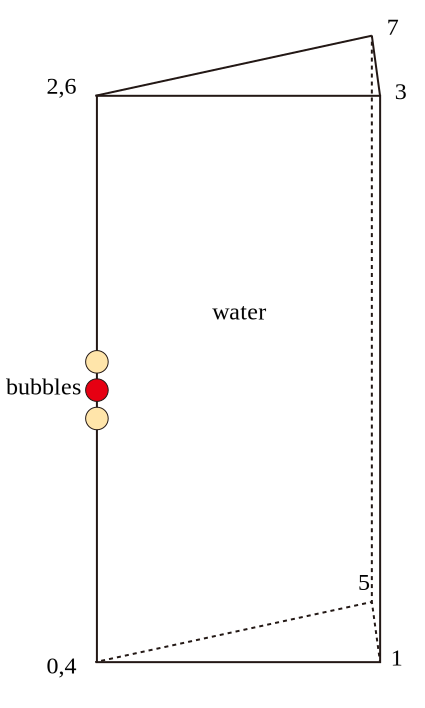
\includegraphics[width=0.45\linewidth]{img/fig4.14.pdf}
    \caption[楔形对称计算域。]{楔形对称计算域。点以数字方式标注。空泡以红色表示。在计算域中,(0,
2, 6, 4)设置为旋转对称面,底面(0, 1, 5, 4),顶面(2, 3, 7,
6),外面(1, 3, 7, 5)属性是 patch,前后面(0, 1, 3, 2)、(4, 5, 7,
6)是对称面 wedge。}
    \label{fig:4.14}
\end{figure}

在本章前几节中,实验研究了激光空泡间的相互作用,其呈现出特殊的膨胀和收缩形态。实验中给出的五种典型案例,表现出了不同的膨胀和溃灭机制。我们将这些机制总结为空泡间的抑制作用与初始距离限制的竞争。在距离较远时的弱相互作用,空泡间的推动作用较小而吸引作用较为明显。继而在收缩阶段产生向中心聚集的效果。在间隔距离次远时,空泡间形成一定的拉伸效果,并使空泡的寿命延长。在间隔距离等于两个相互孤立空泡半径和时,在收缩阶段形成较为明显的拉伸效果,并使中心位置的空泡在溃灭时形成较为明显的长条状。在距离更小时,拉伸效果非常明显,存在将中心位置空泡拉断的情况。但在距离足够小时,距离的作用压制了膨胀的推动作用,使空泡的膨胀和收缩都被压制。形成近似空泡合并的效果。
在这些不同机制的相互变化过程中,可能存在着某种突变或者渐变机制。为了更加详细、明确和物理地探究距离对这种线性排列的空泡间相互作用的机制,本节中借助模拟计算,对该问题进行参数研究。也就是$\gamma$以0.1:0.1:2的方式形成20组结果对比。
数值模拟采用如第二章第五节中给出的基于OpenFOAM的算法实现,并对本章中涉及到的案例做如下特殊设置。

在 OpenFOAM
中,通过单层三维网格获得二维网格模式。在本例中,设置为楔形结构,如图
\ref{fig:4.14}所示。其中地面和顶面以及外面三个面设置边界为:压力,''waveTransmissive'',无反射边界;速度,''pressureInletOutletVelocity'',流入流出边界。如此设置可以获得近似自由域的效果。但为了更好的对实验结果进行解析,基于传统的模拟求解设置,也就是计算域的边界距离空泡中心
$20 R_\mathrm{max}$ 以上。这里设置为 $25 R_\mathrm{max}$
,同时也是实验中容器的大小。本节中设置的情景并不完全对应于实验结果,而是更理想化的自由域情景,比如实验中存在水域的硬边界和软边界,在本节中统一设置为自由域边界。
本节构造了如图 \ref{fig:4.15}
的计算域。为了减少计算时间和提高计算精度,空泡区域的网格密度设置较高,并构成阶梯形式减少的正方形(六面体)结构化网格。在初始生成的计算域中,空泡计算域的网格密度为
$X*Y=(250/5\,\mathrm{mm})*(250/5\,\mathrm{mm})=50*50\,\mathrm{(mm}^{-1})^2$。

\begin{figure}[H]
    \centering
    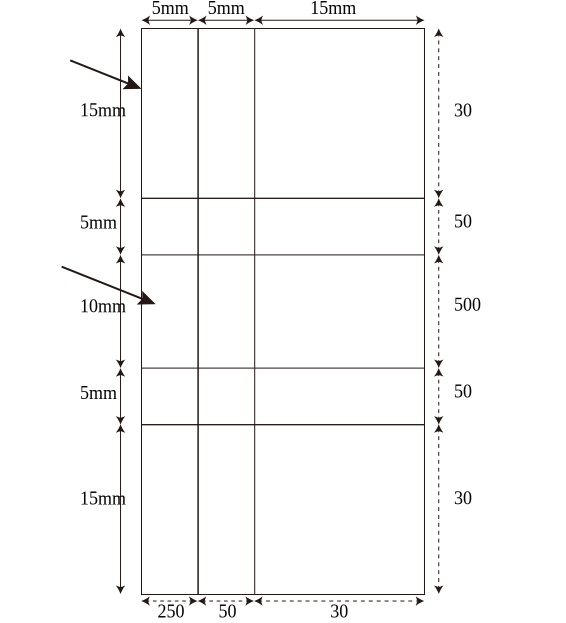
\includegraphics[width=0.5\linewidth]{img/fig4.15.pdf}
    \caption[二维网格划分正面图。]{二维网格划分正面图。计算域尺寸标注在左侧与顶部。对应尺寸划分网格数量标注在右侧和底部。从而获得在图中空泡区域均匀的
0.02mm 网格尺寸。}
    \label{fig:4.15}
\end{figure}


而空泡区域的网格尺寸 $20\,\mathrm{\mu m}$ ,
相比空泡的最小泡半径(初始泡半径
$34\,\mathrm{\mu m}$)处于同一数量级。这不足以精确的追踪空泡的脉动。通常要求最小泡半径时有\textasciitilde100
左右个网格。本文中采取更加极端的选择,即在空泡的脉动区域形成更小的网格尺寸。为此针对空泡区域做了四次网格细化,每次细化将
$X$ 和 $Y$ 方向上 2
倍密度,也就是一个正方形网格变成四个正方形网格。具体到不同 $\gamma$
值,则如图 \ref{fig:4.16} 中所示,形成四次细化。最核心部分的网格密度可以达到
$X*Y=50*50\,\mathrm{(mm}^{-1})^2*(2*2*2*2)^2=800*800\,\mathrm{(mm}^{-1})^2$。也就是最小网格尺寸为
$1.25\,\mathrm{\mu m}<1/20*R_\mathrm{init}=1.7\,\mathrm{\mu m}$。如此的设置后,不同的
$\gamma$
案例,其网格总数量不太一致,但总体每个计算域有\textasciitilde{}
$2\times 10^6$ 个单元格。

\begin{figure}[H]
    \centering
    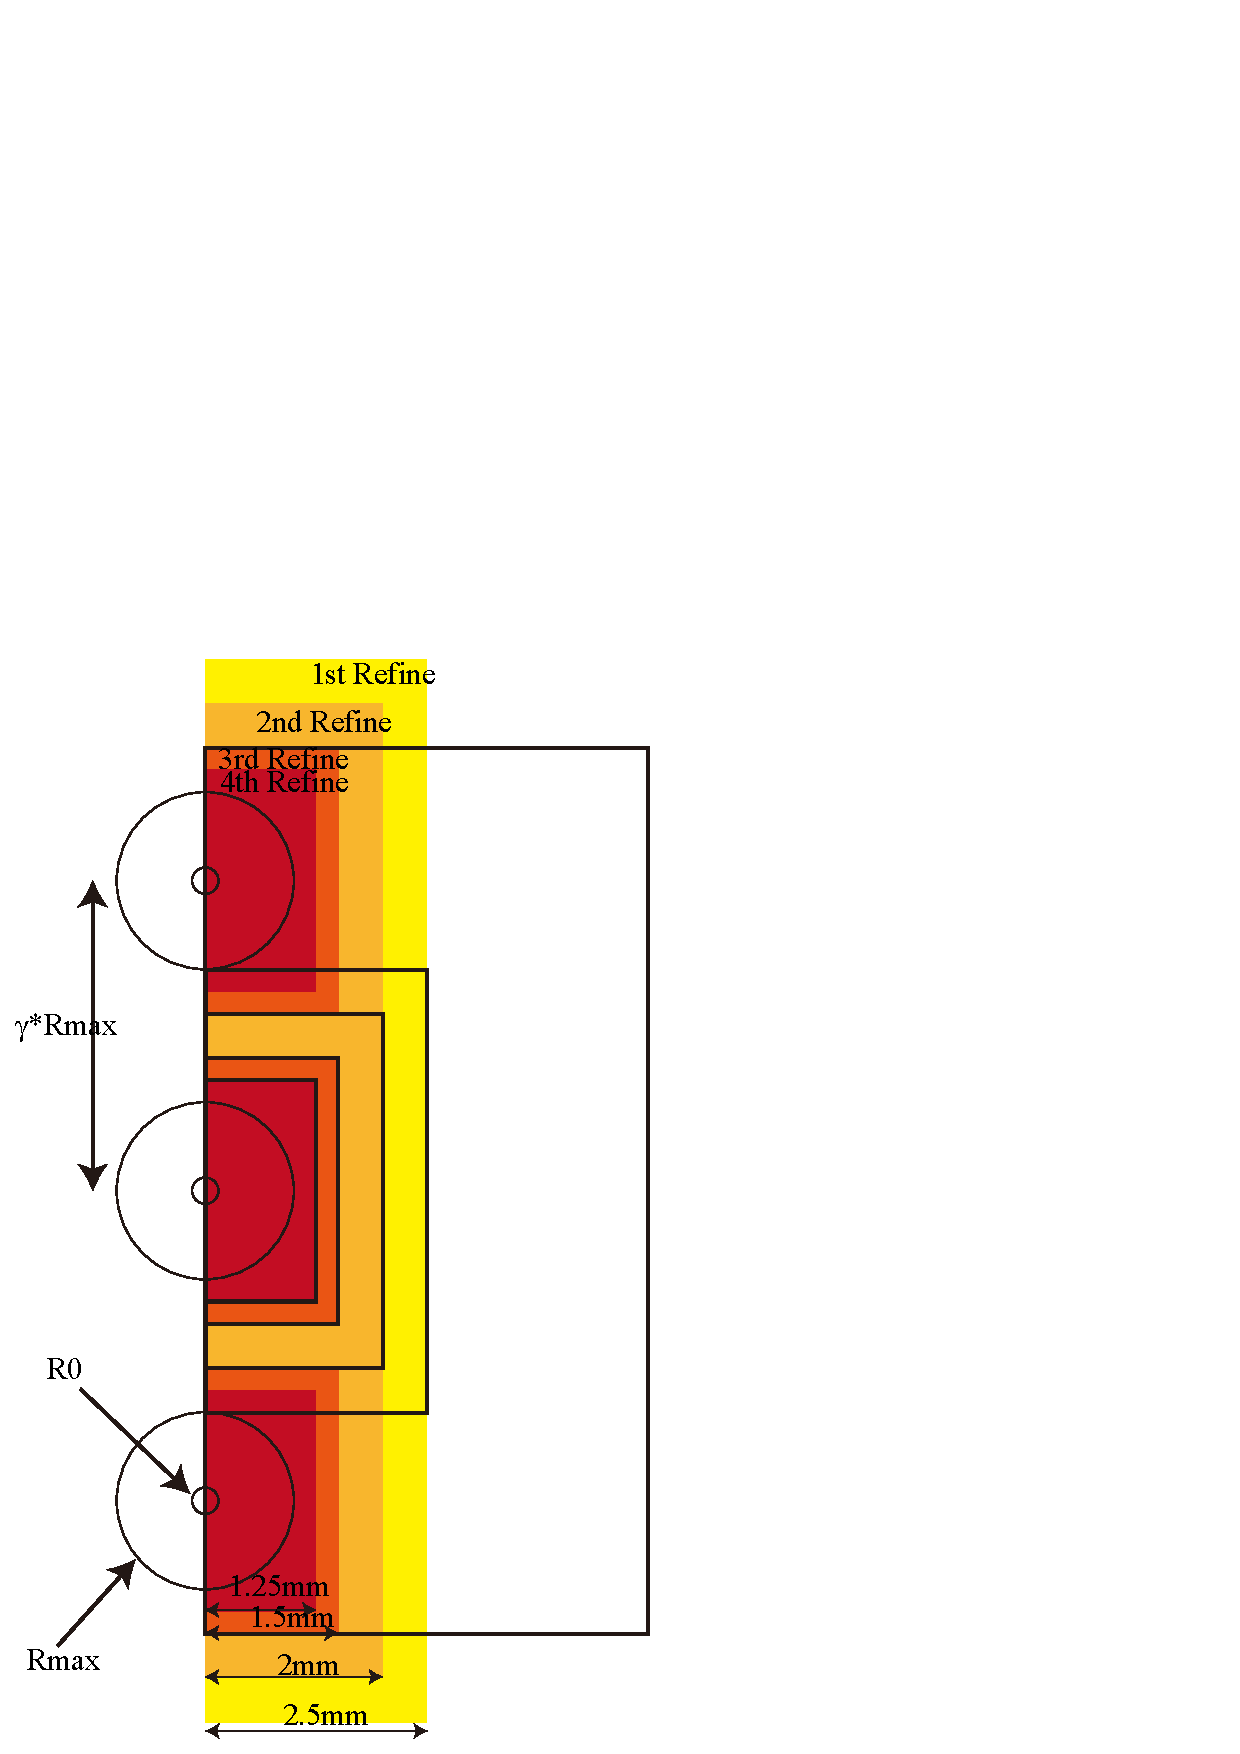
\includegraphics[width=0.6\linewidth]{img/fig4.16.pdf}
    \caption[]{对图中空泡区域的细化,如图中所示。细化顺序由颜色从浅至深标注。其中第一次细化范围是每个空泡中心的
2.5mm 边长的正方形,第二次细化 2mm,第三次细化 1.5mm,第四次细化
1.25mm。在相同的细化过程中,如果三个空泡周围的细化范围有所重叠,则细化范围取其范围并集。}
    \label{fig:4.16}
\end{figure}


\subsection{线性对称排列的三空泡的仿真}
上述的 20
组模拟中,模拟结果表现出较好的规律性,也揭示了一些实验难以获得的信息。上文中实验给出的五组
$\gamma$ 值,其对应的模拟结果相云图如图 \ref{fig:4.17}所示。

\begin{figure}[H]
    \centering
    \includegraphics[width=0.8\linewidth]{img/fig4.17.png}
    \caption[模拟的线性对称排列的三空泡气相云图]{模拟的线性对称排列的三空泡气相云图。通过计算域对其对称轴对称获得。}
    \label{fig:4.17}
\end{figure}


在如上图所示的模拟结果中,较好的获得了空泡间相互作用的过程。与实验结果类似,模拟获得的三空泡阵列膨胀收缩过程中的拉伸和挤压效果突出。通过二维计算所展现的结果,需要绕对称轴旋转才能展现实验中获得的阴影效果。

模拟结果中,对现象的解释此处与上文相符,不再赘述。
在实验中我们根据空泡在溃灭后的破碎残余气体团,推断空泡之间存在着一定程度上的间隔,并据此将空泡分割。在模拟结果中,我们可以观察到,空泡在膨胀期间其水膜稳定存在,但在收缩期间,取决于
$\gamma$
值,水膜过薄时会因拉伸效应和张力的共同作用使水膜断裂成间断排列在原水膜位置上的小液滴。通常这种现象被称为接合(coalescence)。在上述的模拟结果中,这种现象发生在
$\gamma\leq 0.6$
情景下的收缩期间。水膜断裂时通常会在空泡边缘形成凹陷,这是空泡接触所形成的特殊结构,我们仍然可以拓扑的分辨各个空泡的主体。特别地,在
$\gamma\leq 0.4$
时,因空泡间距过近,空泡在膨胀阶段就挤压水膜形成断裂,在最大半径时就完成接合。如此三空泡表现为近异形单空泡的脉动。
另外值得关注的问题是中间空泡的溃灭方式。在线性对称排列的三空泡中,边缘空泡的溃灭方式相互类似,同时也类似于近壁面空泡溃灭,也就是产生自近自由面指向近受约束面的射流导致溃灭。在实验中,我们基于现有的实验结果,以及对空泡控制的不确定性,认为主导中间空泡形成三种溃灭方式的主要原因在于边缘空泡的挤压作用与拉伸作用的斗争。这点是基于学界现有认知和有限的实验结果所获得的科学结论。但在模拟中,因条件的设置更加理想化,使结果中另一种特殊的可能存在的机制暴露出来。也就是在上文的讨论中提到的,在中间空泡收缩过程中,因自身收缩形成射流,或边缘空泡的射流刺穿边缘空泡后进入中间空泡。在相对方向前进的射流,在接近中间空泡的中心位置处相互撞击后,向射流发展的正交的方向延展,在空泡形成自内而外的水相体,使中间空泡自中间层断裂,形成类似拉断的效果。

上一节中提出的三种中间空泡的溃灭机制:1. 拉长; 2. 拉断;3.
上下挤压。其中 2.
拉断合并了上述射流撞击机制可以为断裂机制。针对这三种机制(拉长,断裂,挤压),选取其代表案例的压力和速度场的云图如图
4.18 所示。

\begin{figure}[H]
    \centering
  
    \subfigure[]{
    \includegraphics[width=0.3\linewidth]
    {img/fig4.18a.png}
    
    }
    \subfigure[]{
    \includegraphics[width=0.3\linewidth]
    {img/fig4.18b.png}
    
    }
    \subfigure[]{
    \includegraphics[width=0.3\linewidth]
    {img/fig4.18c.png}
    }
    \caption[三种空泡溃灭机制的压强-相态-速度云图。]{三种空泡溃灭机制的压强-相态-速度云图。
A 显示了挤压机制,其对应 $\gamma=0.5$。图 4.18B
显示了断裂机制,其对应 $\gamma=0.9$。图 4.18C 显示了拉长机制,其对应
$\gamma=1.5$。}
    \label{fig:4.18}
\end{figure}


 在图 \ref{fig:4.18}~.A
中,第一帧显示了边缘空泡开始收缩,但中间空泡仍在膨胀期的压力-相-速度图。可以看到空泡在接触面处延展。第二帧显示了三个空泡都进入了收缩其时的状态,可以看到泡外水体较为均匀的流向空泡区域,并且在边缘空泡内部,主要与对称轴平行地流向空泡接触面。这也就造成了在后期形成碟状结构,即在空泡的主轴长度保持较高长度,而次轴形成溃灭。第三帧中,三个空泡继续收缩,但上述平行的运动趋势仍然存在。第四帧中边缘空泡的射流进入空泡阵列内部。第五帧射流撞击,并形成向外的内生水体,此时空泡内部压强仍小于环境压强,且水体速度仍指向空泡阵列。第六帧显示了如实验图中溃灭末期的景象,水体主要在空泡排列方向流向空泡内部,即挤压模式下的碟形溃灭。

在图\ref{fig:4.18}~.B
中,第一帧显示了射流形成并向阵列内运动的情景。此时中间泡的长度因为距离较大形成的空泡间适度拉伸而形成较大的长度。第二帧显示了三个空泡持续收缩,边缘空泡形成的射流指向中间空泡的内部。第三帧显示,相对射流进入中间空泡内部,中间空泡的外壁仍在收缩但射流附近形成向外的趋势。第四帧显示射流撞击并产生向外延展的水体。第五帧,射流持续撞击,内生外延水体撞击中间空泡外壁。第六帧中,在边缘空泡的牵拉和内生水体的共同作用下,中间空泡自中间破裂。也就是上述的断裂机制。

在简要的图 \ref{fig:4.18}~.C
中,第一帧展现了射流贯穿边缘空泡,中间空泡在被拉长的基础上收缩。中间空泡主要受正交于阵列排列方向的推动。第二帧中,边缘空泡的射流接触中间空泡,更强的流动促使中间空泡在正交方向上收缩。第三帧中中间空泡收缩到射流撞击前刻,可以看到速度达到了
250
m/s。第四帧中,空泡溃灭至极小,正交方向的水体与射流撞击,产生较高的本地压力可以达到
$5.8\times 10^7 Pa$。这种形成正交高速水体与边缘射流撞击的溃灭形式,就是上文中的拉长机制。

更宏观地,统计了 20 组不同 $\gamma$ 值的内外空泡的溃灭时间,以研究
$\gamma$
对内外空泡溃灭形式的影响。因为空泡的不对称溃灭,在空泡生存末期,不会有一个体积极小的瞬间,而是在射流刺穿后逐渐破碎,故而本文中将边缘空泡的射流到达相对面的瞬间作为空泡的溃灭时间,并将中间空泡的射流相对接触时当作空泡的溃灭时间。即空泡被液体贯穿(penetrated)的时刻当作空泡的溃灭时刻。而不是过度的追踪残余气体的脉动。
内外空泡的溃灭时间受 $\gamma$ 影响的曲线如图 \ref{fig:4.19} 所示。

\begin{figure}[H]
    \centering
    \includegraphics[width=0.8\linewidth]{img/fig4.19.png}
    \caption{不同间距条件下内外空泡被射流击穿的时间对比。}
    \label{fig:4.19}
\end{figure}


在图 \ref{fig:4.19}中,可以看到 $\gamma$
越小,也就是空泡间距越小,边缘空泡受其他空泡的影响越大,边缘空泡的溃灭时间越大。在图中,对应的孤立单空泡的生存时间是
$183\mathrm{\mu s}$,也就是无穷远处, $\gamma$
极大时,其溃灭时间会趋向于 $183\mathrm{\mu s}$。与之相反地,在
$\gamma \leq 1.2$ 时, $\gamma$
越大中间空泡溃灭时间越长。这是因为在这段区间,空泡间的拉伸效应将中间空泡持续拉伸,边缘空泡的射流进入中间空泡的路径增长,碰撞时间变长。同时因距离增大,中间空泡的膨胀时间更长,膨胀更加充分,也推迟了其溃灭时间。在
$\gamma>1.2$
时,因泡间相互作用减弱,拉伸效果也减弱,造成溃灭时间减小。特殊地,在
$\gamma \leq 0.6$ 时,空泡在溃灭阶段形成一个大的接合空泡,在
$\gamma \leq 0.4$
时空泡在膨胀阶段就接合成一个大空泡。在这个区间,空泡接合,一般的,间距越近,其相互作用越强越早,接合成一个大空泡的能量越高,持续的时间越久。

同时,为了量化的反映空泡溃灭机制,定义一个参数,空泡溃灭瞬间的长短轴比,
$$
\chi  =\frac B A  =\frac {Y_\mathrm{end}} {X_\mathrm{end}} 
$$
此处 $A$、$B$ 的定义如上文中给出,在模拟中,我们固定的将 $A$ 与
$X_\mathrm{end}$、$B$ 与 $Y_\mathrm{end}$ 等效,即模拟中空泡在 x-y
轴上的边界值就是主次轴长。$\chi<1$ 时,溃灭的形态偏挤压, $\chi>1$
时,溃灭的形态偏拉伸。下图中(图 4.20)给出了不同 $\gamma$
值下的中间空泡的 $\chi$ 值。

\begin{figure}[H]
    \centering
    \includegraphics[width=1\linewidth]{img/fig4.20.png}
    \caption[空泡溃灭时的长短轴。]{空泡溃灭时的长短轴。A
给出了分别在边缘或者中间空泡被穿刺时的中间空泡主次轴长比。B
则给出了对应的情景下的主次轴长度。}
    \label{fig:4.20}
\end{figure}


从图 \ref{fig:4.20}中可以看到, $\chi$ 在 $\gamma=1.4$ 时获得最大,也就是在
$\gamma=1.4$ 时获得最好的拉伸效果。在 $\gamma=0.9$ 时获得
$\chi\approx 1$ ,也就是其溃灭时主次轴比约为
1,具有较好的圆性,可以形成较强烈的溃灭效果。同时,可以发现,在
$\gamma>1.4$
时,溃灭时的主轴长度几乎不发生变化,由此可知在此情景下,无穷远处对空泡的影响趋同,泡间相互作用影响其拉伸效果。在
$\gamma<1.4$
时,因为泡间相互作用造成在泡间阵列排列位置上的挤压和正交方向上的延展,遗留到溃灭阶段形成其交叉形状。

\section{本章总结}

在本章,实验和数值研究了均匀分离的三个激光致空泡的动力学。实验中,利用光学全息法在三维准自由水域获得特定排布的多点激光击穿,并借此在水中获得击穿空泡。精密控制的距离和能量实现了较为理想化条件下的单生命周期内的多空泡的相互作用。$\gamma$
作为均匀分布的多空泡间距的参数,在本研究中作为主要研究参数。

1.在阵列空泡中,空泡的生存时间普遍延长,体积变小。这种现象因中间泡受到的抑制最明显而使中间泡最为突出。在溃灭时,这种生存时间差使空泡的溃灭从外到内有序进行。同时,$\gamma$越小这种现象越明显。

2.空泡的不同部位的不同相位延迟造成了空泡的特殊形状。以一种相对独立的视角来看,可以认为,一个空泡内部部分,距相邻空泡越近的部分其相位推迟越大。这种现象是通过空泡与空泡脉动的声辐射相互作用来实现。
声辐射使空泡内外压差产生变化,在相应的脉动阶段对继续运动产生抑制效果,从而使空泡产生的相位推迟。

3.同相位等间距的三空泡系统中,中间空泡的溃灭形态有多种:不受影响,稍微在排列方向上拉长,拉长至长条状,沙漏状,和被压缩的碟型。中间泡不产生射流,两边向中间射流并且随着
  $\gamma$
  值的减小而变得强烈。一般地表示空泡形状稳定性的参数------圆性的开始失去可以发生在任意阶段,并随着
  $\gamma$ 减小而向前移动,从溃灭末期直到初生阶段。


4.在空泡阵列脉动期间,空泡通过声辐射相互作用,泡能转移使相对位置变动。在膨胀期,边缘空泡被向外推动。在收缩期则牵拉边缘空泡向内移动。$\gamma$越小,这种效果越明显。

在本章中利用多个参数来描述空泡的相互作用。未来需要有更进一步的描述相互作用过程中形变的参数。需要对生命周期的延长进行量化。对空泡能量的去向有更准确的计量。同时要改进实验方法,以期获得更准确的相互作用中空泡内部的信息。

